\documentclass[tikz,border=2pt]{standalone}
\usepackage{amsmath,amssymb}
\usepackage{pgfplots}
\pgfplotsset{compat=1.18}
\usetikzlibrary{arrows.meta}

\begin{document}
% f(x) = x^3 - 3x^2 + 3 with its tangent at x0 = 1.5: f(1.5) = -0.375, f'(1.5) = -2.25,
% tangent y = -2.25x + 3.
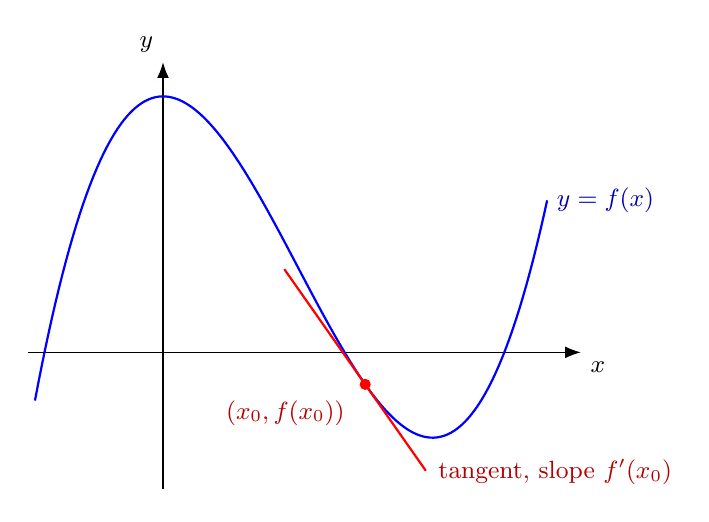
\begin{tikzpicture}[every node/.style={font=\small}]
	\begin{axis}[
		width=8.6cm, height=7cm,
		axis lines=middle, axis line style={-{Latex[length=2mm]}},
		xmin=-1, xmax=3.1, ymin=-1.6, ymax=3.4,
		xtick=\empty, ytick=\empty,
		tick label style={font=\small},
		xlabel={$x$}, ylabel={$y$},
		xlabel style={below right}, ylabel style={above left},
		samples=150, clip=false
		]
		\addplot[blue, thick, domain=-0.95:2.85] {x^3-3*x^2+3};
		\addplot[red, thick, domain=0.9:1.95] {-2.25*x+3};
		\addplot[only marks, mark=*, mark size=1.8pt, red] coordinates {(1.5,-0.375)};
		\node[red!70!black, anchor=north east, font=\small] at (axis cs:1.42,-0.45) {$(x_0,f(x_0))$};
		\node[blue!70!black, anchor=west] at (axis cs:2.85,{2.85^3-3*2.85^2+3}) {$y=f(x)$};
		\node[red!70!black, anchor=west] at (axis cs:1.97,-1.4) {tangent, slope $f'(x_0)$};
	\end{axis}
\end{tikzpicture}
\end{document}
